\newcommand{\econtexRoot}{.}

\documentclass[\econtexRoot/HAFiscal]{subfiles}
\onlyinsubfile{\externaldocument{\econtexRoot/HAFiscal}} % Get xrefs -- esp to apndx -- from main file; only works if main file has already been compiled

\begin{document}

\addcontentsline{toc}{section}{Appendices} % label the section "Appendices"

\hypertarget{Appendices}{} % Allows link to [url-of-paper]#Appendices
\ifthenelse{\boolean{Web}}{}{% Web version has no page headers
  \chead[Appendices]{Appendices}      % but PDF version does
  \appendixpage % Reset formatting for appendices
} 

\hypertarget{Estimating-discount-factor-distributions-for-different-interest-rates}{}\par\section{Estimating discount factor distributions for different interest rates}
\notinsubfile{\label{app:DF_R}}



Figure~\ref{fig:LorenzPtsrobustnessR} shows the fit of the liquid wealth distribution for interest rates of $0.5$ percent and $1.5$ percent per quarter. In both cases, the estimation exactly matches the median liquid wealth to permanent income ratios for each education group listed in Panel~B of Table~\ref{tab:estimBetas}. 

% \begin{table}{th}
%   \begin{center}
%     \begin{tabular}{lccc}
        %         \multicolumn{4}{l}{Panel (B) Estimation targets} \\ \midrule
        %         & Dropout & Highschool & College \\ \midrule
        %         Median LW/PI (data) & 4.64 & 30.2 & 112.8 \\ 
        %         Median LW/PI (model, $R = 1.005$) & 4.64 & 30.2 & 112.8 \\	
        %         Median LW/PI (model, $R = 1.01$) & 4.64 & 30.2 & 112.8 \\
        %         Median LW/PI (model, $R = 1.015$) & 4.64 & 30.2 & 112.8 \\ \bottomrule
        %       \end{tabular} \\ \\ 
        %         \end{center}	
        %         \end{table}

\begin{figure}[th]
  \begin{center}
    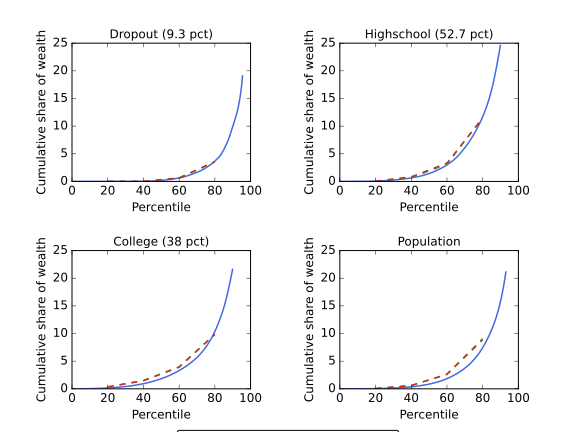
\includegraphics[width=.9\textwidth]{\econtexRoot/Figures/LorenzPoints_robustness_R}
    \caption{Distributions of liquid wealth within each educational group and for the whole population from the 2004 Survey of Consumer Finance and from the estimated model for different values of the interest rate, $R$.}
    \notinsubfile{\label{fig:LorenzPtsrobustnessR}}
  \end{center}
\end{figure}



\FloatBarrier

\hypertarget{Model_without_splurge}{}\par\section{Results in a model without the splurge}
\notinsubfile{\label{app:Model_without_splurge}}

In this appendix, we reestimate the model in the absence of the splurge. We discuss that model's ability to match (targeted and untargeted) empirical targets in the Norwegian and US setting. We then use the reestimated model to asses the relevance of the splurge for the effectiveness of the three policies. 


\subsection{Estimating discount factor distributions in the absence of the splurge}

For the purpose of evaluating the results in the model without the splurge we do not require the reestimation of our Norwegian model, as the purpose of the latter is the estimation of the splurge. Nevertheless, we test wether we match the IMPC as reported by \citet{fagereng_mpc_2021} when the splurge is zero. Figure \ref{splurge0_Norwayestimation} illustrates the fit when we impose the splurge to be zero in comparison to our baseline estimation. 

\begin{figure}[htb]
	\centering
	\begin{subfigure}[b]{.48\linewidth}
		\centering
		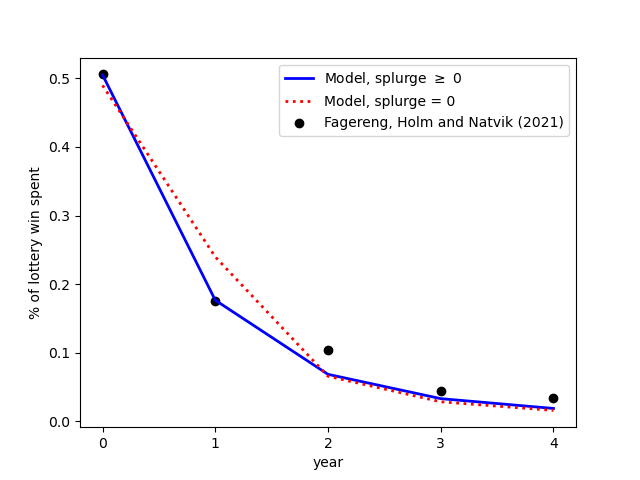
\includegraphics[width=\linewidth]{\econtexRoot/Code/HA-Models/Target_AggMPCX_LiquWealth/Figures/AggMPC_LotteryWin_comparison_splurge0}
		\caption{Share of lottery win spent}
		\notinsubfile{\label{fig:aggmpclotterywin}}
	\end{subfigure}
	\begin{subfigure}[b]{.48\linewidth}
		\centering
		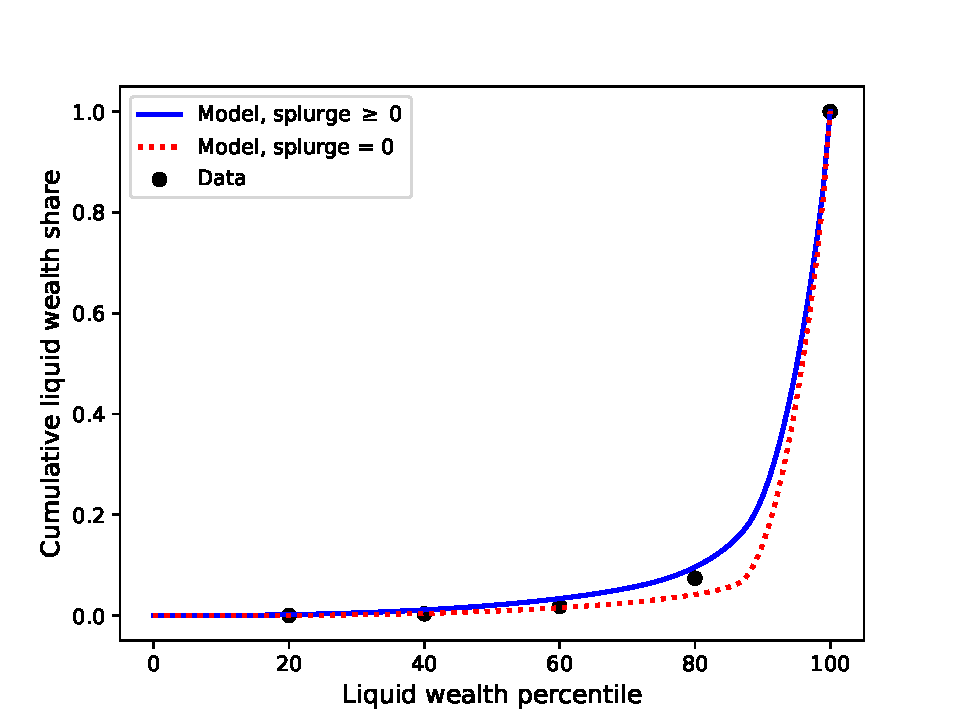
\includegraphics[width=\linewidth]{\econtexRoot/Code/HA-Models/Target_AggMPCX_LiquWealth/Figures/LiquWealth_Distribution_comparison_splurge0}
		\caption{Distribution of liquid wealth}
		\notinsubfile{\label{fig:liquwealthdistribution}}
	\end{subfigure}%
	\caption{Targets and model moments from the estimation}
	\notinsubfile{\label{fig:splurge0_Norwayestimation}}
	\parbox{16cm}{\small \vspace{.15cm} \textbf{Note}: Panel (a) shows the fit of the model to the dynamic consumption response estimated in \citet{fagereng_mpc_2021}; see their figure~A5. Panel (b) shows the fit of the model to the distribution of liquid wealth (see Section~\ref{sec:SCFdata} for the definition) from the 2004 SCF.\normalsize}
\end{figure}

While the splurge helps in matching the empirical evidence on the IMPC, the model without the splurge performs also relatively well. This is because the model without the splurge is able to generate a high initial marginal propensity to consume through a wider distribution of discount factors ($\beta = 0.921$ and $\nabla=0.116$) relative to the model with a splurge ($\beta = 0.968$ and $\nabla=0.0578$). This ensures that sufficiently many agents are at the borrowing constraint and thus sensitive to transitory income shocks. However, this comes at the cost of a loss in the fit of the distribution of liquid wealth, which is now more unequal relative to the baseline case with a positive splurge and the data. The model without the splurge also does not perfectly match the dynamics of the marginal propensity to consume over time. Specifically, the model exhibits a higher spending propensity in the first year after the shock as borrowing-constrained agents spend the additional income quicker. 

Also, the fit with respect to other moments deterioriates. While the model with the splurge can account for empirically-observed initial MPCs among the wealthiest, the model without the splurge exhibits much lower MPCs among that group, see Table \ref{tab:Comparison_Splurge_Table}. Overall, the model fit with the data deteriorates roughly by a factor of two measured by the Euclidean norm of the targeting error.\footnote{Specifically, the Euclidean norm of the targeting error increases from 0.04 to 0.08 for the time-profile of the marginal propensity to consume when the splurge is removed, from 0.16 to 0.29 for the marginal propensity to consume across wealth quartiles and from 0.027 to 0.032 for the Lorentz curve.} 



\begin{table}[t]
	\center
	\begin{tabular}{@{}lcccccc@{}} 
\toprule 
                  & \multicolumn{5}{c}{MPC} &   \\   
                  &  1st WQ  & 2nd WQ  & 3rd WQ & 4th WQ  & Agg  &  K/Y  \\  \midrule 
Splurge $\geq$ 0 &0.27 & 0.48 & 0.60 & 0.66 & 0.50 & 6.58 \\ 
Splurge = 0 &0.13 & 0.51 & 0.62 & 0.68 & 0.49 & 6.59 \\ 
Data &0.39 & 0.39 & 0.55 & 0.66 & 0.51 & 6.60 \\ 
\end{tabular}  

	\caption{Marginal propensities to consume across wealth quartiles and the total population as well as the wealth to income ratio, in the model with and without the splurge and according to the data}
	\notinsubfile{\label{tab:Comparison_Splurge_Table}}
\end{table}







We now turn to the estimation of the discount factor distributions in the US calibration of the model when the splurge is absent. \\
\\
XXX\\
FOR HAKON\\
estimation results of discout factors when splurge = 0\\
discuss initial MPCs and iMPC / liquid wealth fit when splurge = 0 relative to splurge > 0\\
XXX\\


It is also instructive to compare the consumption dynamics of agents experiencing longer spells of unemployment in the model with and without the splurge. This can be seen in figure \ref{fig:UIextension_CompSplurge0}, which plots the evolution of income, consumption and share of agents at the borrowing limit among those that stay unemployed for at least five quarters. In this simulation there is no recession and none of the fiscal policies are implemented. While the consumption dynamics across the models with and without the splurge are fairly similar, the underlying drivers of the consumption drop upon expiry of unemployment benefits are different. In the model with the splurge, the drop in income translates directly in lower consumption via the splurge itself. In the model without the splurge it is the sharp rise in agents hitting the borrowing constraint which accounts for the consumption drop after UI benefits expire. This is due to the wider distribution of discount factors in the model without the splurge, which leads to a greater number of agents close the borrowing constraint. 


\begin{figure}[t]
	\centering
	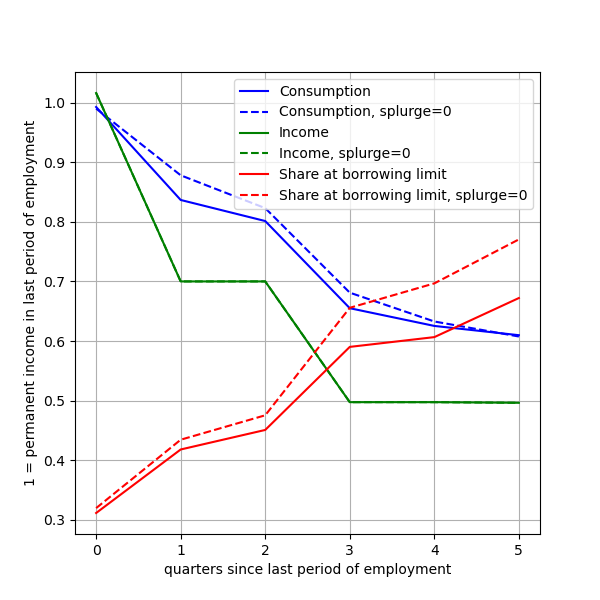
\includegraphics[width=0.8\linewidth]{Code/HA-Models/FromPandemicCode/Figures/Splurge0/UIextension_CompSplurge0}
	\caption{Consumption and income levels for agents staying unemployed for at least five quarters and the share of those agents at the borrowing limit, in the model with and without the splurge. Note: No policy nor the recession are active.}
	\notinsubfile{\label{fig:UIextension_CompSplurge0}}
\end{figure}


\FloatBarrier
\subsection{Multipliers in the absence of the splurge}

In this section we simulate the three fiscal policies from the main text in the estimated model without the splurge. The shape of the impulse response functions only marginally change relative to the model with the splurge. Hence, we focus on the quantitative changes as summarized by the cummulative multipliers in Figure \ref{fig:cumulativemultipliers_SplurgeComp}. The figure shows the multipliers when AD effects are switched on for the model with and without the splurge. Table \ref{tab:Multiplier_SplurgeComp} shows the 10y-horizon multiplier across the two models.

The absence of the splurge entails a calibration with a lower average MPC in the population. Hence, the check and tax cut exhibit lower multipliers when there is no splurge. For the UI extension we observe the opposite pattern, as the multiplier is larger in the model without the splurge. This due to the consumption dynamics around the expiry of UI benefits described in the previous section. In the model without the splurge more agents hit the borrowing constraint upon the expiry. Providing those agents with an extension of UI benefits thus turns out slightly more powerful. 

The policy ranking in terms of the multiplier shifts slighlty. While viewed from the model with the splurge, the check policy delivers multiplier effects much more rapidly than the UI extension, the UI extension appears superior to the check in the model without the splurge, both at shorter as well as longer horizons. Both models agree on the tax cut being the least effective policy. 

\begin{figure}[t]
	\centering
	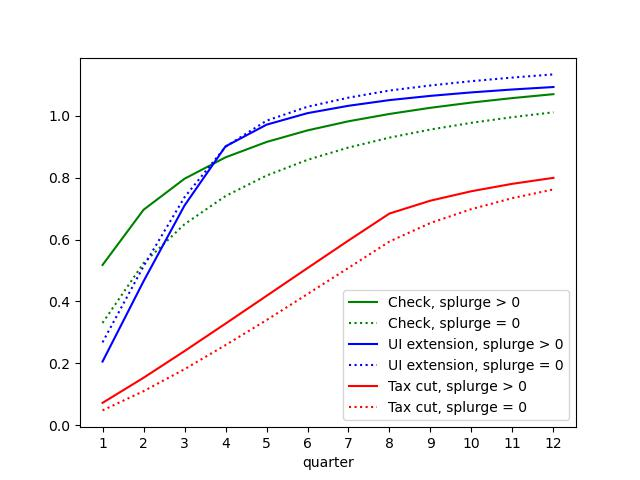
\includegraphics[width=0.8\linewidth]{Code/HA-Models/FromPandemicCode/Figures/Splurge0/Cummulative_multipliers_SplurgeComp}
	\caption{Cumulative multiplier as a function of the horizon for the three policies with and without the splurge. Note: Policies are implemented during a recession with AD effect active.}
	\notinsubfile{\label{fig:cumulativemultipliers_SplurgeComp}}
\end{figure}


\begin{table}[t]
	\center
	\begin{tabular}{@{}lccc@{}} 
\toprule 
& Stimulus check    & UI extension    & Tax cut     \\  \midrule 
10y-horizon Multiplier (no AD effect)  &0.870(0.854)  & 0.910(0.893)  & 0.839(0.826)     \\ 
10y-horizon Multiplier (AD effect) &1.143(1.199)  & 1.221(1.175)  & 0.947(0.952)     \\ \bottomrule
\end{tabular}  

	\caption{Multipliers, calculated for policies implemented in a recession with and without aggregate demand effects. The values outside of the brackets capture the multipliers in the model without the splurge, while those inside the brackets are the corresponding mulitipliers with the splurge.}
	\notinsubfile{\label{tab:Multiplier_SplurgeComp}}
\end{table}





%\subfile{Robustness}
\subfile{HANKAppendix}

\ifthenelse{\boolean{Web}}{}{
\end{document} \endinput
}

